\documentclass[12pt,a4paper]{article}
\usepackage[utf8]{inputenc}
\usepackage{graphicx}
\usepackage{lmodern}
\usepackage[T1]{fontenc}
\usepackage[italian]{babel}
\usepackage{hyperref}
\usepackage{amsmath} 
\usepackage{algorithm}
\usepackage{algorithmic}
\usepackage{changepage}
\usepackage{adjustbox}
\usepackage{tikz}
\usetikzlibrary{shapes.geometric, arrows}


\title{\textbf{Progetto: Heuristics \& Metaheuristics for Optimization \& Learning}}
\author{
    Nome Cognome\\
    Matricola: 000000\\
    Corso di Laurea in Informatica\\
    Università degli Studi di Catania
}
\date{Luglio 2025}

\begin{document}

\begin{titlepage}
    \centering
    
    {
\includegraphics[width=3cm]{sigillo-2014.png}\par} 
    \vspace{1cm}

    {\Large Università degli Studi di Catania\par}
    {\large Dipartimento di Matematica e Informatica\par}
    \vspace{2cm}

    {\LARGE\bfseries Progetto Heuristics \& Metaheuristics for Optimization \& Learning\par}
    \vspace{1.5cm}

    {\Large Relazione Finale\par}
    \vspace{2cm}

    {\Large Prof. Mario Pavone\par}
    \vspace{1cm}

    {\Large Studente: Matteo Vullo\par}
    {\Large Matricola: 1000034661\par}
    \vfill

    {\large Luglio 2025\par}
\end{titlepage}

\tableofcontents
\newpage

\section{Introduzione}

Il problema del massimo flusso (\textit{Maximum Flow Problem}) è uno dei classici problemi della teoria dei grafi e dell’ottimizzazione combinatoria.

Formalmente, dato un grafo diretto $ G = (V, E) $ con capacità positive associate a ciascun arco, il problema consiste nel determinare il flusso massimo che può essere inviato da un nodo sorgente $ s $ ad un nodo pozzo $ t $, rispettando le capacità degli archi e la conservazione del flusso nei nodi intermedi.

In questo progetto è stato implementato un algoritmo metaeuristico per la risoluzione del problema del massimo flusso. L’obiettivo principale è stato progettare, implementare e testare un algoritmo capace di raggiungere soluzioni vicine all’ottimo in tempi ragionevoli.

\section{Scelta dell'Algoritmo}

Tra le molteplici metaeuristiche disponibili per la risoluzione del problema del massimo flusso (\textit{Maximum Flow Problem}), è stato scelto di implementare l'algoritmo \textit{Tabu Search} (TS). Questa decisione si basa su una serie di motivi tecnici e strategici che rendono Tabu Search particolarmente adatto al contesto del problema affrontato.

Uno dei motivi principali è la capacità del Tabu Search di evitare il blocco in ottimi locali, grazie all’utilizzo della \textit{lista tabù}, una struttura di memoria a breve termine che impedisce la ripetizione di mosse recenti. Questo è un aspetto cruciale nel contesto del massimo flusso, dove piccole variazioni locali del flusso possono portare a soluzioni apparentemente ottimali ma non globali.

Un secondo fattore decisivo è la flessibilità nella definizione del vicinato e delle mosse,che si adatta bene alla struttura del problema. Nel progetto, sono state implementate diverse tipologie di mosse che operano direttamente sugli archi del grafo permettendo di bilanciare esplorazione e intensificazione in base alle caratteristiche del grafo.

Un aspetto non trascurabile è il punto di partenza della ricerca. L’algoritmo parte da una soluzione iniziale di alta qualità. Questo garantisce una base solida per la ricerca locale e riduce il numero di iterazioni necessarie per convergere verso il valore ottimo.

Infine, Tabu Search offre un buon compromesso tra complessità di implementazione e capacità di esplorazione dello spazio di ricerca, risultando una scelta originale e adatta al problema specifico. La sua applicazione nel contesto del massimo flusso, pur non essendo comune, si è dimostrata efficace, producendo risultati molto vicini a quelli ottimali calcolati con algoritmi esatti

\section{Implementazione dell'Algoritmo}

L'implementazione dell'algoritmo Tabu Search (TS) per il problema del massimo flusso è stata progettata per essere efficiente, modulare e conforme ai requisiti sperimentali. L'intera logica è stata strutturata in una classe principale, \texttt{MaxFlowTabuSearch}, che incapsula le operazioni principali: inizializzazione del grafo, generazione della soluzione iniziale, ricerca locale, gestione della memoria tabu, diversificazione e valutazione della funzione obiettivo.

\subsection{Struttura della Soluzione}
Ogni soluzione rappresenta un vettore $ \vec{f} \in \mathbb{R}^n $, dove $ n = |E| $, e ogni componente $ f_i $ indica il flusso sull’arco $ i $-esimo.

\subsection{Funzione Obiettivo}
La funzione obiettivo nel problema del massimo flusso rappresenta il valore totale del flusso inviato dalla sorgente al pozzo. Essa è definita come la somma dei flussi sugli archi uscenti dalla sorgente $ s $:

$$
f_{\text{tot}} = \sum_{(s, v) \in E} f(s, v)
$$

\subsection{Inizializzazione della Soluzione}
L'inizializzazione della soluzione rappresenta un passo cruciale nell'algoritmo Tabu Search, in quanto determina il punto iniziale da cui parte la ricerca. Una buona inizializzazione permette di ridurre il tempo di convergenza e migliorare la qualità della soluzione finale.

\subsubsection{Inizializzazione Casuale}
Questa strategia genera una soluzione iniziale casuale, rispettando i vincoli di capacità di ogni arco. Il flusso iniziale su ogni arco $ (u,v) $ è estratto uniformemente nell’intervallo $ [0, c(u,v)] $, dove $ c(u,v) $ è la capacità dell’arco.

Questa strategia è semplice e veloce, ma può comportare una maggiore variabilità tra le esecuzioni e un tempo di convergenza più lungo, soprattutto per grafi complessi.  Usata come baseline, non adottata come strategia principale.

\subsubsection{Inizializzazione Greedy}
La strategia greedy cerca di costruire una soluzione iniziale sfruttando un approccio costruttivo: vengono identificati percorsi aumentanti dal nodo sorgente al pozzo e viene spinto il massimo flusso possibile lungo questi percorsi, fino a un numero limitato di iterazioni.

L’algoritmo utilizza una variante di Dijkstra per trovare il percorso aumentante con la capacità residua massima.

Questa strategia mira a bilanciare velocità e qualità iniziale, fornendo una soluzione migliore di quella casuale senza richiedere il calcolo completo del flusso ottimo.

\subsubsection{Inizializzazione EK parziale}
La soluzione iniziale è stata costruita utilizzando una versione parziale dell'algoritmo \texttt{Edmonds-Karp}, un algoritmo esatto per il calcolo del massimo flusso. Questo algoritmo è stato utilizzato per ottenere una soluzione ottima parziale, che è stata successivamente ridotta proporzionalmente con un fattore casuale $ r \in [0.7, 0.95] $, in modo da non fornire direttamente la soluzione ottima ma una base promettente per la ricerca locale.

Formalmente:
\[
f_{\text{iniziale}}(u,v) = f_{\text{Edmonds-Karp}}(u,v) \cdot r
\]
dove:

    
- $ f_{\text{Edmonds-Karp}}(u,v) $: flusso calcolato con l'algoritmo esatto.
    
- $ r $: fattore di riduzione casuale.

Questa strategia di inizializzazione riduce significativamente il rischio di partire da una configurazione non ammissibile o troppo distante dalla soluzione ideale, migliorando la stabilità e la coerenza della ricerca. Inoltre, il fatto di non dover "partire da zero" permette all’algoritmo di convergere più rapidamente verso il valore ottimo, riducendo il numero di iterazioni necessarie e aumentando l’efficienza complessiva del processo di ricerca.

Tra le diverse strategie di inizializzazione testate la migliore si è rivelata senza dubbio l’inizializzazione EK parziale. Tutte le mosse e le strategie successive (vicinato, diversificazione, adattività) sono state quindi testate e applicate a partire da questa soluzione iniziale, rendendola il fondamento su cui si basa l’efficacia complessiva dell’algoritmo.

\subsection{Definizione delle Mosse}

Le mosse nell'algoritmo Tabu Search implementato rappresentano variazioni locali del flusso sugli archi del grafo, con l'obiettivo di migliorare progressivamente il valore totale del flusso dal nodo sorgente al nodo pozzo, rispettando i vincoli di capacità e conservazione del flusso.

\subsubsection{Mosse Elementari (Incremento/Decremento del Flusso)}

Le \textit{mosse elementari} consistono nel modificare il flusso su un singolo arco $(u, v)$ aumentandolo o riducendolo di una quantità $\delta$, rispettivamente, purché non si violino i vincoli di capacità.

Formalmente, una mossa elementare è definita come:
\[
f'(u,v) = 
\begin{cases} 
f(u,v) + \delta & \text{se } f(u,v) + \delta \leq c(u,v) \\
f(u,v) - \delta & \text{se } f(u,v) - \delta \geq 0
\end{cases}
\]
dove:

    
- $ f(u,v) $: flusso attuale sull'arco $ (u,v) $;
    
- $ c(u,v) $: capacità dell'arco $ (u,v) $;
    
- $ \delta $: passo di modifica del flusso, scelto come il minimo tra il 20\% della capacità residua o il 20\% della capacità totale.

Queste mosse permettono un’intensificazione locale del processo di ricerca invece il passo del 20\% della capacità (residua o totale) bilancia aggressività e stabilità, evitando oscillazioni eccessive. Inoltre sono applicate ogni iterazione, garantendo una continua ottimizzazione

Di seguito è riportato lo pseudocodice per la generazione di una mossa elementare:

\begin{algorithm}[H]
\caption{Mosse Elementari}
\label{alg:elementary_moves}
\begin{algorithmic}[1]
\REQUIRE $\texttt{current\_flow}$: vettore del flusso corrente.
\REQUIRE $\texttt{edge\_idx}$: indice dell'arco da modificare.
\ENSURE $\texttt{new\_flow}$: nuova soluzione con la mossa applicata.

\STATE $ c \gets \texttt{capacities[edge\_idx]} $
\STATE $ f \gets \texttt{current\_flow[edge\_idx]} $

\IF{$ f < c $}
    \STATE $ \delta \gets \min(c - f, 0.2 \cdot c) $
    \STATE $ \texttt{new\_flow} \gets \texttt{current\_flow} $
    \STATE $ \texttt{new\_flow[edge\_idx]} \gets f + \delta $
    \STATE $ \texttt{is\_tabu} \gets \texttt{edge\_idx in tabu\_list} $
    \RETURN $\texttt{new\_flow}, \texttt{is\_tabu}$
\ELSIF{$ f > 0 $}
    \STATE $ \delta \gets \min(f, 0.2 \cdot c) $
    \STATE $ \texttt{new\_flow} \gets \texttt{current\_flow} $
    \STATE $ \texttt{new\_flow[edge\_idx]} \gets f - \delta $
    \STATE $ \texttt{is\_tabu} \gets \texttt{edge\_idx in tabu\_list} $
    \RETURN $\texttt{new\_flow}, \texttt{is\_tabu}$
\ENDIF
\RETURN \texttt{None} (nessuna mossa applicabile)
\end{algorithmic}
\end{algorithm}

\subsubsection{Mosse di Scambio tra Archi (Edge Exchange)}

Le \textit{mosse di scambio tra archi} sono utilizzate per redistribuire il flusso da archi saturi (o quasi saturi) verso archi poco utilizzati. Questo tipo di mossa è applicato ogni 20 iterazioni ed è utile per evitare che l’algoritmo si blocchi in ottimi locali.

Formalmente, dati due archi $ (u_1, v_1) $ e $ (u_2, v_2) $, con flusso $ f_1 $ e $ f_2 $, e capacità $ c_1 $ e $ c_2 $, si applica:
\[
\begin{aligned}
f'_1 &= f_1 - \Delta \\
f'_2 &= f_2 + \Delta
\end{aligned}
\]
dove $ \Delta = \min(f_1, c_2 - f_2) $, garantendo che i vincoli di capacità siano rispettati.

Queste mosse rompono gli stalli causati da archi bloccati, reintroducendo flessibilità.
Operano in modo mirato trasferendo il flusso da un arco quasi pieno a uno con capacità residua.

Ecco lo pseudocodice per la generazione di una mossa di scambio:

\begin{algorithm}[H]
\caption{Mosse di Scambio tra Archi}
\label{alg:edge_exchange_moves}
\begin{algorithmic}[1]
\REQUIRE $\texttt{current\_flow}$: vettore del flusso corrente.
\ENSURE $\texttt{new\_flow}$: nuova soluzione con la mossa applicata.

\STATE $ \texttt{saturated} \gets [i \mid i \in \texttt{edges}, \texttt{current\_flow}[i] \geq \texttt{capacity}[i] - \epsilon] $
\STATE $ \texttt{unsaturated} \gets [i \mid i \in \texttt{edges}, \texttt{current\_flow}[i] < \texttt{capacity}[i] - \epsilon] $

\IF{not $\texttt{saturated}$ or not $\texttt{unsaturated}$}
    \RETURN \texttt{None}
\ENDIF

\STATE $ \texttt{src} \gets \texttt{random.choice(saturated)} $
\STATE $ \texttt{dest} \gets \texttt{random.choice(unsaturated)} $
\STATE $ \Delta \gets
\min(\texttt{current\_flow[src]}, \texttt{capacity[dest]} - \texttt{current\_flow[dest]}) $

\IF{ $\Delta \leq \epsilon $ }
    \RETURN \texttt{None}
\ENDIF

\STATE $ \texttt{new\_flow} \gets \texttt{current\_flow} $
\STATE $ \texttt{new\_flow[src]} \gets \texttt{new\_flow[src]} - \Delta $
\STATE $ \texttt{new\_flow[dest]} \gets \texttt{new\_flow[dest]} + \Delta $

\RETURN $\texttt{new\_flow}$
\end{algorithmic}
\end{algorithm}

\subsubsection{Mosse di Aumento su Cammino (Path Augmentation)}

Le \textit{mosse di aumento su cammino} sono ispirate al classico algoritmo di Edmonds-Karp. Vengono utilizzate periodicamente o in caso di stallo, per cercare un cammino aumentante dal nodo sorgente al nodo pozzo nel grafo residuo.

Se un cammino aumentante viene trovato, il flusso lungo quel cammino viene incrementato del massimo valore possibile, in base alla capacità residua minima lungo gli archi del cammino. Questo permette di migliorare il flusso globale in modo significativo.

Queste mosse permettono miglioramenti globali significativi , superando ottimi locali.
Sono applicate ogni 100 iterazioni o in caso di stallo, per limitarne il costo computazionale

Ecco lo pseudocodice per la generazione di una mossa di aumento su cammino:

\begin{algorithm}[H]
\caption{Mossa di Aumento su Cammino}
\label{alg:path_augmentation_move}
\begin{algorithmic}[1]
\REQUIRE $\texttt{current\_flow}$: vettore del flusso corrente.
\ENSURE $\texttt{new\_flow}$: nuova soluzione con la mossa applicata.

\STATE $ \texttt{path} \gets \texttt{find\_augmenting\_path(current\_flow)} $
\IF{ $\texttt{path is None} $ }
    \RETURN \texttt{None}
\ENDIF

\STATE $ \Delta \gets \min(\texttt{capacity}[e] - \texttt{current\_flow}[e] \mid e \in \texttt{path}) $
\STATE $ \texttt{new\_flow} \gets \texttt{current\_flow} $
\FOR{ogni arco $ e \in \texttt{path} $}
    \STATE $ \texttt{new\_flow}[e] \gets \texttt{new\_flow}[e] + \Delta $
\ENDFOR

\RETURN $\texttt{new\_flow}$
\end{algorithmic}
\end{algorithm}

\subsection{Memoria Tabù}

Nell'implementazione dell'algoritmo \textit{Tabu Search}, la lista tabù è stata realizzata non come una semplice lista o insieme, ma come un \texttt{dizionario} chiamato \texttt{tabu\_dict}, in cui ogni chiave è l'indice di un arco e il valore associato è il numero di iterazione fino al quale quell'arco rimane ``tabù'':

\[
\texttt{tabu\_dict} = \{ \texttt{indice\_arco}: \texttt{iterazione\_fine\_tabù} \}
\]

Il dizionario è stato utilizzato per tre ragioni principali:

- \textbf{Accesso rapido}: grazie alla struttura hash interna di Python, verificare se un arco è tabù avviene in tempo costante $O(1)$, fondamentale quando si analizzano centinaia o migliaia di mosse candidate.
    
    
- \textbf{Gestione temporale precisa}: a differenza di una semplice flag booleana, il dizionario permette di memorizzare \textit{fino a quando} un arco è vietato. Questo consente di applicare correttamente la \texttt{tabu\_tenure} senza dover scandire continuamente la cronologia delle mosse.

    
- \textbf{Facilità di aggiornamento e pulizia}: ogni volta che si modifica un arco, si inserisce (o si sovrascrive) la sua scadenza. Inoltre, ogni 500 iterazioni, gli elementi scaduti possono essere rimossi facilmente:
    \[
    \texttt{tabu\_dict = \{k: v for k, v in tabu\_dict.items() if v > iteration\}}
    \]
    Questo mantiene la memoria leggera e le prestazioni stabili nel tempo.


L’utilizzo del dizionario permette di evitare sia i cicli ripetitivi (grazie al blocco temporaneo delle mosse inverse), sia di mantenere il costo computazionale di ricerche lineari.
    
Di seguito è riportato lo pseudocodice che mostra come viene utilizzata la \texttt{tabu\_dict} nella selezione della miglior mossa.

\begin{algorithm}[H]
\caption{Utilizzo della Memoria Tabù nella Selezione della Mossa}
\label{alg:tabu_usage}
\begin{algorithmic}[1]
\REQUIRE $\texttt{moves}$: lista di mosse candidate.
\REQUIRE $\texttt{best\_value}$: valore della miglior soluzione globale.
\ENSURE $\texttt{best\_move}$: mossa selezionata.

\STATE $\texttt{best\_val} \gets -\infty$
\STATE $\texttt{best\_move} \gets \texttt{None}$

\FOR{ogni mossa in $\texttt{moves}$}
    \STATE $(\texttt{new\_flow}, \texttt{idx}) \gets \texttt{mossa}$
    \STATE $\texttt{is\_tabu} \gets (\texttt{idx} \in \texttt{tabu\_dict}) \land (\texttt{tabu\_dict[idx]} > \texttt{iteration})$

    \IF{$\texttt{not is\_tabu OR calculate\_flow(new\_flow)} > \texttt{best\_value}$}
        \STATE $\texttt{val} \gets \texttt{calculate\_flow(new\_flow)}$
        \IF{$\texttt{val} > \texttt{best\_val}$}
            \STATE $\texttt{best\_val} \gets \texttt{val}$
            \STATE $\texttt{best\_move} \gets (\texttt{new\_flow}, \texttt{idx})$
        \ENDIF
    \ENDIF
\ENDFOR

\STATE Applica $\texttt{best\_move}$ e aggiorna $\texttt{current\_flow}$
\STATE Aggiungi l'arco modificato a $\texttt{tabu\_dict}$ con scadenza: $\texttt{iteration + tabu\_tenure}$
\IF{$\texttt{iteration} \mod 500 == 0$}
    \STATE Rimuovi da $\texttt{tabu\_dict}$ tutti gli archi con scadenza $\leq \texttt{iteration}$
\ENDIF
\end{algorithmic}
\end{algorithm}

\subsection{Diversificazione}

Per evitare la stagnazione in ottimi locali, ogni 2000 iterazioni senza miglioramenti significativi viene applicata una perturbazione alla soluzione corrente. Questa diversificazione combina:

    
- una riduzione proporzionale del flusso globale (moltiplicato per un fattore casuale in $[0.6, 0.8]$);
    
- l’aggiunta di rumore su un sottoinsieme limitato di archi (al più 5 o il 5\% del totale), con variazioni in $[-0.2 \cdot c(u,v), 0.2 \cdot c(u,v)]$.

Questa operazione avviene rispettando i vincoli del problema, in modo da mantenere sempre una soluzione ammissibile:
\[
f'(u,v) = 
\begin{cases} 
f(u,v) \cdot (1 - r) & \text{con } r \in [0.6, 0.8] \\
f(u,v) + \delta & \text{con } \delta \in [-0.2 \cdot c(u,v), 0.2 \cdot c(u,v)]
\end{cases}
\]

Le operazioni rispettano i vincoli di capacità e conservazione del flusso, garantendo una soluzione sempre ammissibile. Questa strategia reintroduce variabilità senza ripartire da zero, favorendo un’efficace esplorazione di nuove regioni dello spazio di ricerca.

\subsection{Adattività dei Parametri}

Per bilanciare esplorazione e intensificazione, la \texttt{tabu\_tenure} è aggiornata dinamicamente in base al \texttt{stagnation\_counter}, che misura le iterazioni senza miglioramenti:

\[
\texttt{tabu\_tenure} = 
\begin{cases} 
\min(t \cdot 1.2, 150) & \text{se stagnazione } > 100 \\
\max(t \cdot 0.9, 10)  & \text{se stagnazione } < 50
\end{cases}
\]

Un valore più alto di \texttt{tabu\_tenure} favorisce l’esplorazione in caso di stallo, mentre uno più basso intensifica la ricerca attorno a soluzioni promettenti. Questa adattività migliora la robustezza dell’algoritmo su istanze di diverse dimensioni.

\subsection{Selezione del Vicinato e Criterio di Aspirazione}

La selezione della mossa ottimale avviene in due fasi: generazione di un \textbf{vicinato ridotto} e applicazione di una \textbf{strategia di accettazione con aspirazione}.

Il vicinato è costruito considerando solo una piccola frazione degli archi (circa l'1–2\% del totale), selezionati casualmente ad ogni iterazione. Questa scelta è motivata da ragioni di efficienza computazionale: un vicinato completo sarebbe troppo costoso da esplorare, specialmente su istanze grandi. Limitandosi a mosse locali mirate, l’algoritmo mantiene tempi di esecuzione ridotti senza sacrificare la qualità della ricerca.

Tra le mosse candidate, viene selezionata quella che massimizza il flusso, purché non sia tabù o soddisfi il \textbf{criterio di aspirazione}: una mossa tabù è comunque accettata se conduce a una soluzione migliore della migliore trovata finora. Questo bilancia esplorazione ed efficacia, evitando di scartare miglioramenti significativi solo per effetto della memoria tabù.

Formalmente:
\[
\text{mossa\_selezionata} = 
\arg\max_{m \in N(s)} 
\left( f(m) \mid m \notin \text{TabuList} \lor f(m) > f(s^*) \right)
\]
dove $ s^* $ è la miglior soluzione globale.

Questa strategia garantisce robustezza e flessibilità, ed è fondamentale per evitare stagnazione e raggiungere soluzioni vicine all’ottimo.

\begin{algorithm}[H]
\caption{Selezione della Miglior Mossa (con Criterio di Aspirazione)}
\label{alg:select_best_move_with_aspiration}
\begin{algorithmic}[1]
\REQUIRE $\texttt{moves}$: lista di mosse candidate.
\REQUIRE $\texttt{best\_value}$: valore della miglior soluzione globale finora trovata.
\ENSURE $\texttt{best\_move}$: la mossa selezionata.

\STATE $\texttt{best\_val} \gets -\infty$
\STATE $\texttt{best\_move} \gets \texttt{None}$

\FOR{ogni mossa in $\texttt{moves}$}
    \STATE $(\texttt{new\_flow}, \texttt{idx}, \texttt{delta}, \texttt{is\_tabu}) \gets \texttt{mossa}$
    \STATE $\texttt{val} \gets \texttt{calculate\_flow\_value(new\_flow)}$

    \IF{$\texttt{is\_tabu}$}
        \STATE \COMMENT{La mossa è tabù, ma può essere accettata se soddisfa il criterio di aspirazione}
        \IF{$\texttt{val} > \texttt{best\_value}$}
            \STATE \texttt{Aggiorna la mossa comunque, grazie al criterio di aspirazione}
        \ELSE
            \STATE \texttt{Salta la mossa (non migliora la soluzione migliore)}
            \STATE \texttt{continua}
        \ENDIF
    \ENDIF

    \IF{$\texttt{val} > \texttt{best\_val}$}
        \STATE $\texttt{best\_val} \gets \texttt{val}$
        \STATE $\texttt{best\_move} \gets (\texttt{new\_flow}, \texttt{idx})$
    \ENDIF
\ENDFOR

\RETURN $\texttt{best\_move}$
\end{algorithmic}
\end{algorithm}

\subsection{Diagramma di flusso}
\begin{figure}[H]
\centering
\begin{tikzpicture}[
    node distance=1.3cm, 
    every node/.style={font=\small},
    box/.style={rectangle, draw, minimum height=0.6cm, text width=2.4cm, align=center}
]
\node (start) [box] {Inizio};
\node (init) [box, below of=start] {Inizializzazione};
\node (moves) [box, below of=init] {Genera vicinato};
\node (select) [box, below of=moves] {Seleziona miglior mossa};
\node (apply) [box, below of=select] {Applica mossa};
\node (update) [box, below of=apply] {Aggiorna lista tabù};
\node (adapt) [box, below of=update] {Adatta parametri};
\node (stop) [box, below of=adapt] {Stop?};
\node (diversify) [box, right of=update, xshift=3cm] {Diversifica};
\node (end) [box, below of=stop, yshift=-0.8cm] {Fine}; 

\draw[->] (start) -- (init);
\draw[->] (init) -- (moves);
\draw[->] (moves) -- (select);
\draw[->] (select) -- (apply);
\draw[->] (apply) -- (update);
\draw[->] (update) -- (adapt);
\draw[->] (adapt) -- (stop);
\draw[->] (stop.east) -| node[above, pos=0.25] {No} (diversify);
\draw[->] (diversify) |- (moves);
\draw[->] (stop.south) -- node[right, pos=0.5] {Sì} (end); 
\end{tikzpicture}
\caption{Diagramma di flusso dell'algoritmo Tabu Search}
\label{fig:flowchart}
\end{figure}

\section{Risultati Sperimentali}

I risultati sperimentali mostrano l’efficacia dell’algoritmo Tabu Search nell’approssimare il valore ottimo del flusso. Di seguito sono riportati i dati aggregati ottenuti su 10 esecuzioni per ciascuna istanza testata.

\begin{table}[ht]
\centering
\begin{adjustbox}{max width=\textwidth}
\begin{tabular}{|l|c|c|c|c|c|c|}
\hline
\textbf{Istanza} & \textbf{Best Flow} & \textbf{Mean Flow ± Std} & \textbf{Avg Iter} & \textbf{Avg Eval} & \textbf{Avg Time (s)} & \textbf{Optimal Flow} \\
\hline
network\_160.txt & 34.68 & 34.68 ± 0.00 & 111 & 3040 & 0.0398 & 34.68 \\
network\_500.txt & 107.98 & 107.98 ± 0.00 & 466 & 15199 & 0.2530 & 107.98 \\
network\_960.txt & 117.74 & 117.74 ± 0.00 & 676 & 911193 & 17.3125 & 117.74 \\
network\_1440.txt & 134.00 & 134.00 ± 0.00 & 1191 & 38422 & 1.3289 & 134.00 \\
network\_2880.txt & 341.00 & 341.00 ± 0.00 & 2601 & 84058 & 5.2702 & 341.00 \\
network\_4320.txt & 555.00 & 555.00 ± 0.00 & 5690 & 184009 & 21.9878 & 555.00 \\
network\_5760.txt & 1203.00 & 1203.00 ± 0.00 & 11132 & 359843 & 101.0931 & 1203.00 \\
network\_7200.txt & 2502.00 & 2484.28 ± 15.97 & 19205 & 640573 & 384.7562 & 2502.00 \\
network\_11520.txt & 1244.00 & 1241.95 ± 6.15 & 11918 & 415316 & 115.9730 & 1244.00 \\
network\_23040.txt & 2223.00 & 2201.18 ± 24.80 & 19147 & 632720 & 379.5599 & 2223.00 \\
\hline
\end{tabular}
\end{adjustbox}
\caption{Risultati aggregati su 10 esecuzioni per tutte le istanze testate.}
\label{tab:risultati_aggregati}
\end{table}

I risultati indicano che l’algoritmo riesce a raggiungere valori molto vicini o uguali all’ottimo teorico, con una deviazione standard nulla o ridotta, evidenziando una buona stabilità e ripetibilità tra le diverse esecuzioni.

\subsection{Grafico di Convergenza}

Per analizzare il comportamento dinamico dell’algoritmo durante l’esecuzione, sono stati generati due tipi principali di grafici:

\subsubsection{Convergenza della Miglior Esecuzione (Best Run)}

Questo tipo di grafico mostra l'andamento del flusso nella migliore esecuzione tra le 10 run effettuate per ogni istanza. La "miglior run" è definita come quella che ha raggiunto il massimo valore di flusso finale.

Il grafico permette di osservare la velocità di convergenza, le fasi di rapido miglioramento e la presenza di stagnazione. Il valore ottimo, calcolato tramite Edmonds-Karp, è indicato da una linea rossa tratteggiata per facilitare il confronto.

\begin{figure}[H]
    \centering
    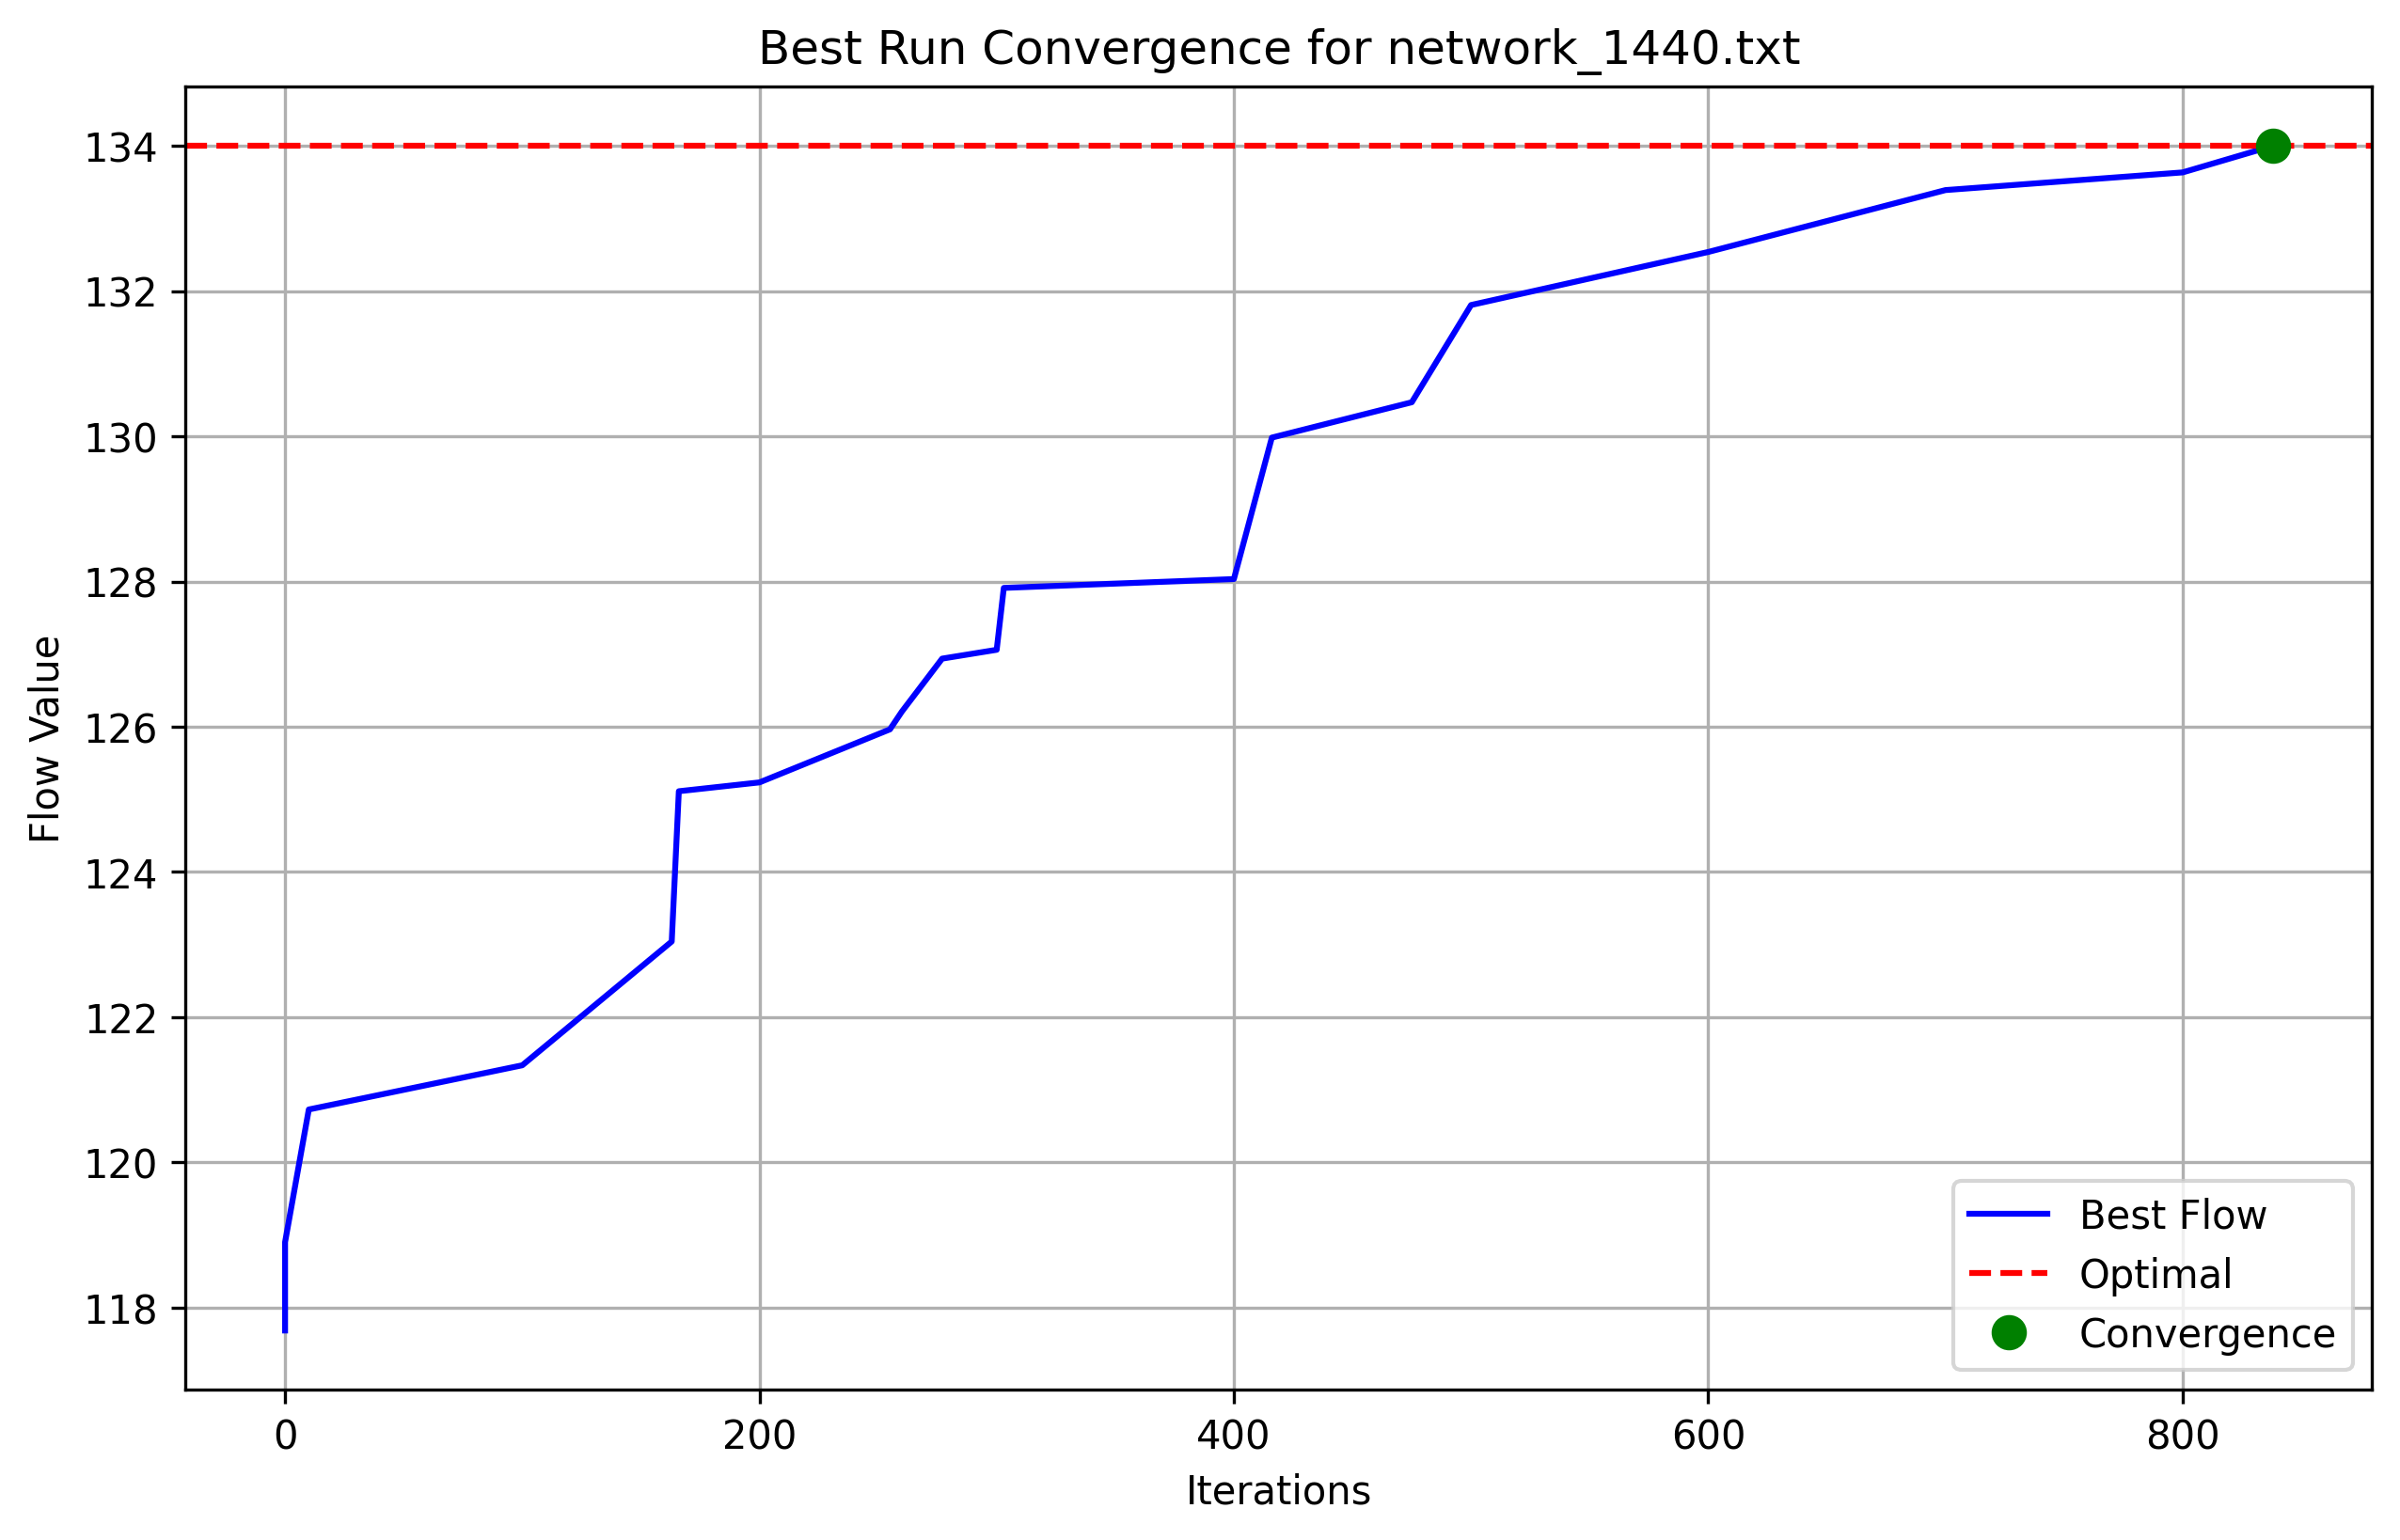
\includegraphics[width=0.8\textwidth]{results/network_1440_best_convergence.png}
    \caption{Convergenza della miglior esecuzione per l'istanza \texttt{network\_1440.txt}.}
    \label{fig:best_run_1440}
\end{figure}

\begin{figure}[H]
    \centering
    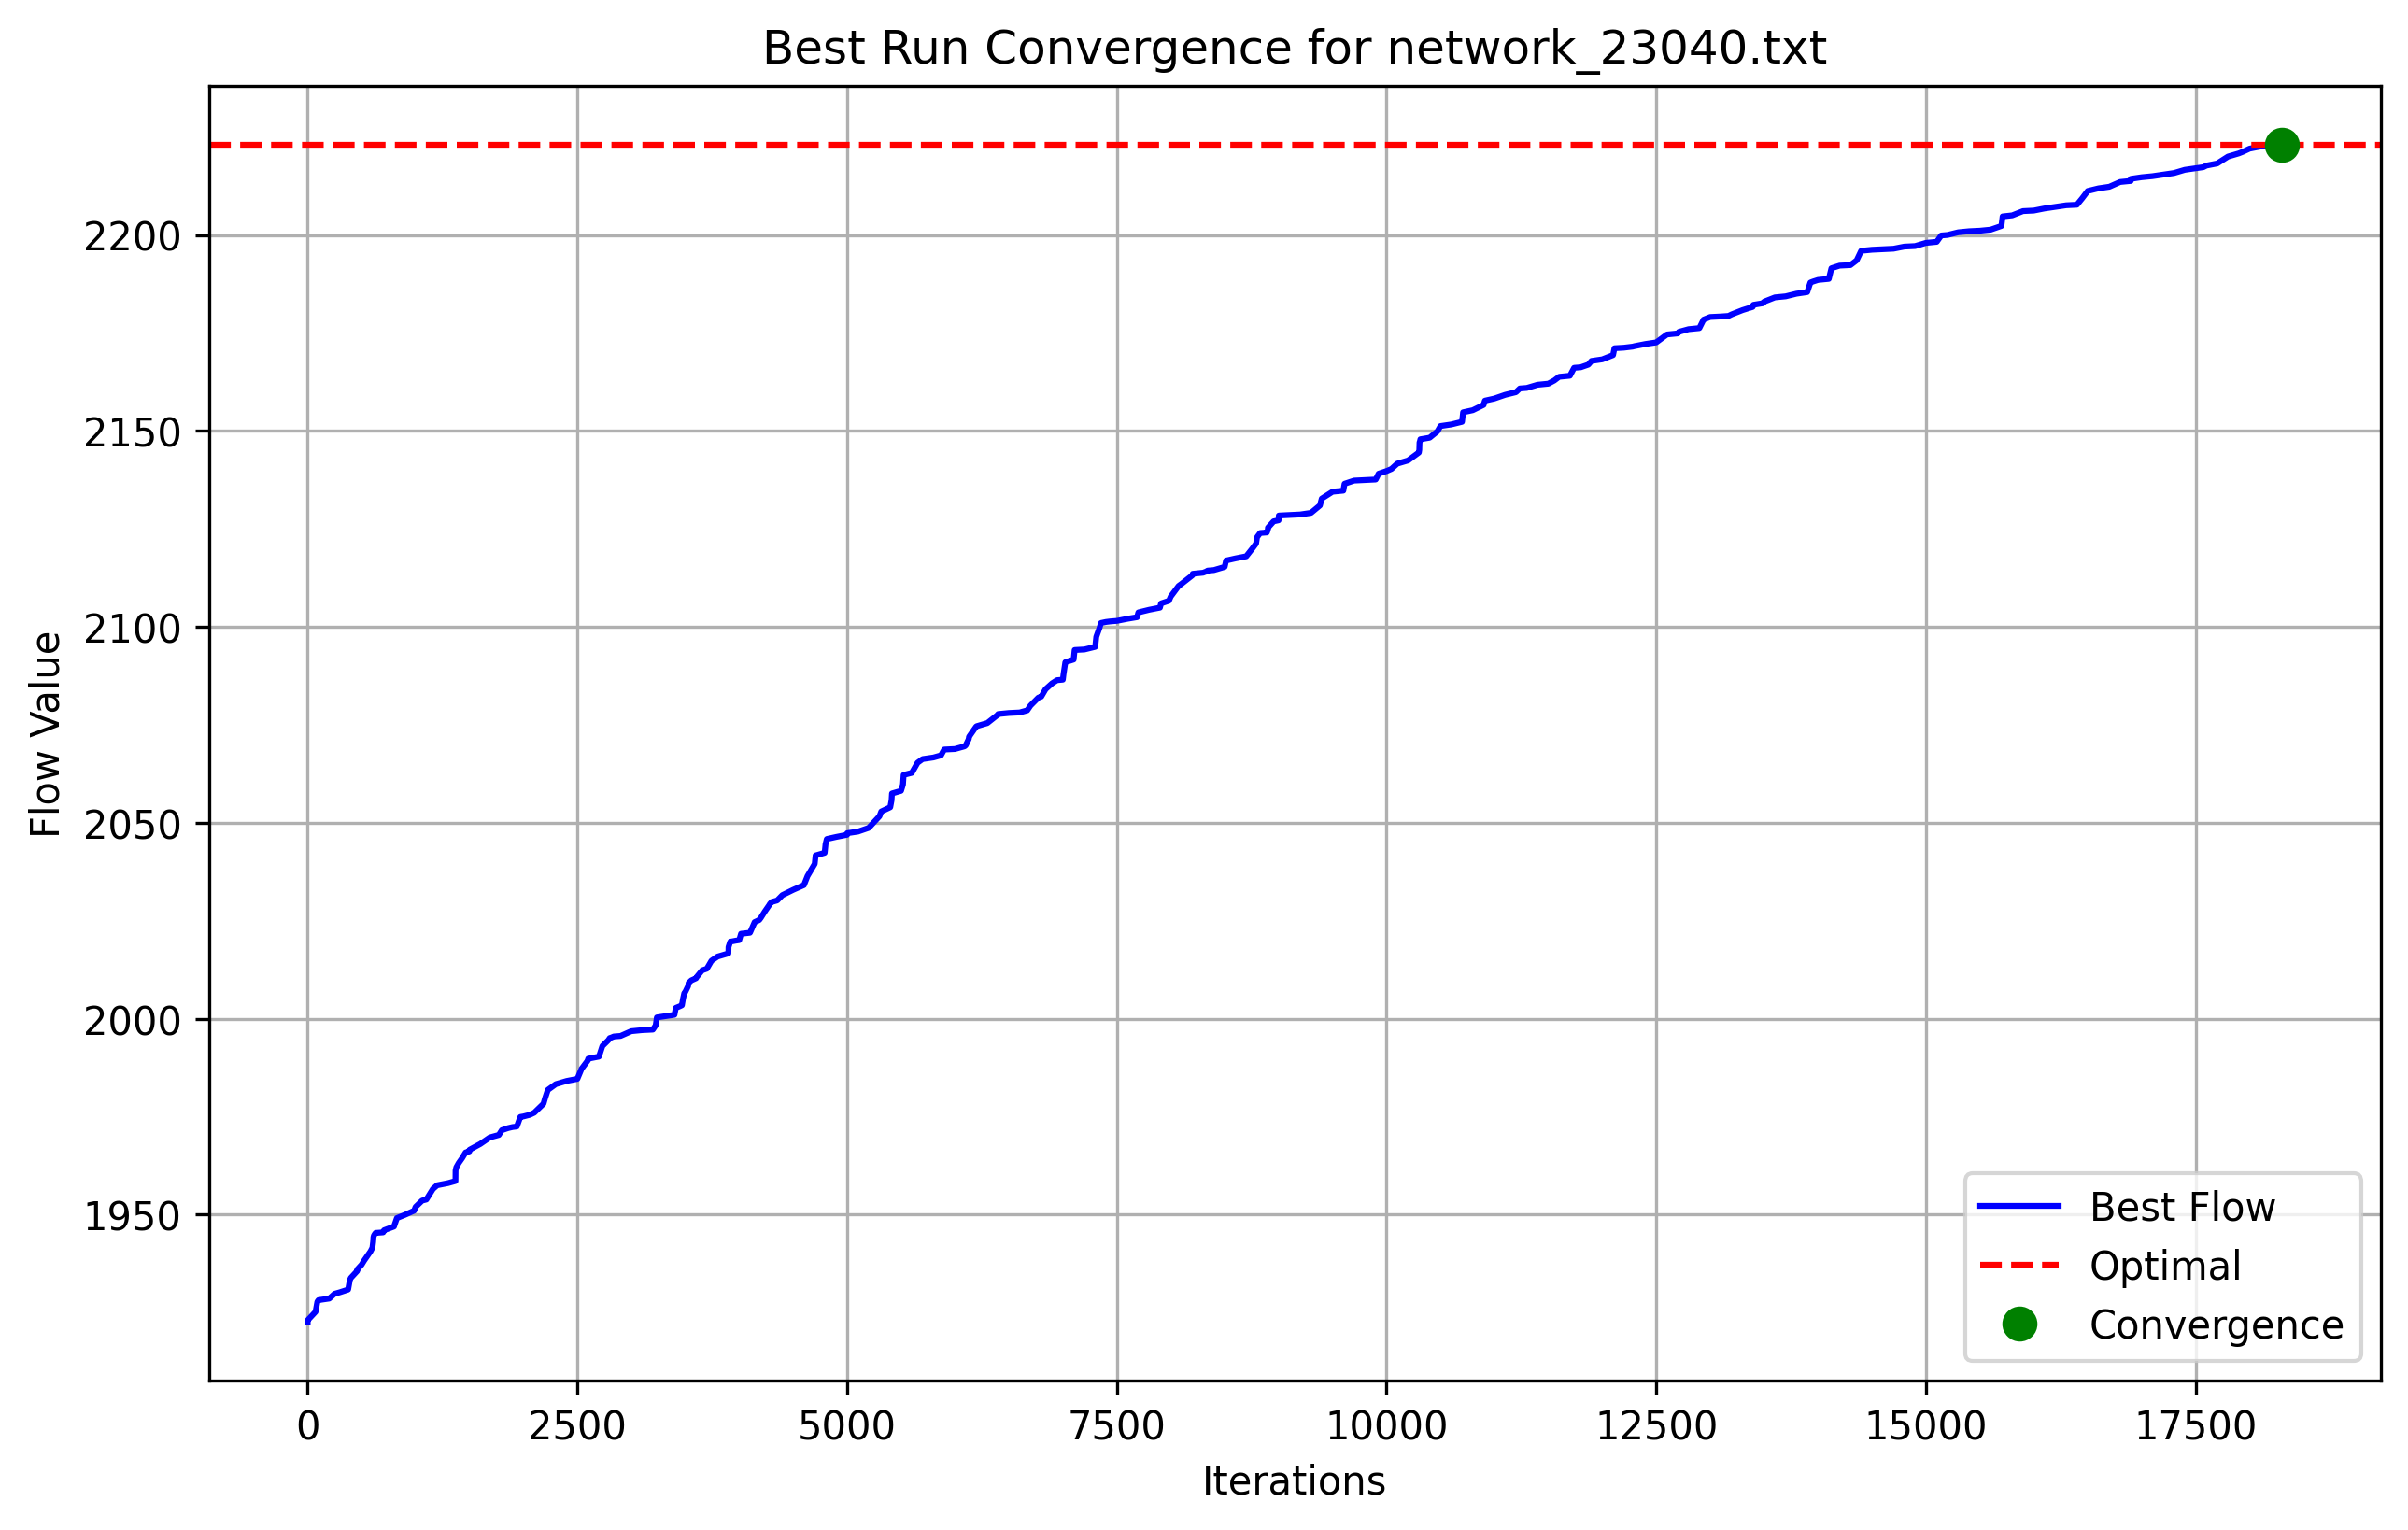
\includegraphics[width=0.8\textwidth]{results/network_23040_best_convergence.png}
    \caption{Convergenza della miglior esecuzione per l'istanza \texttt{network\_23040.txt}.}
    \label{fig:best_run_23040}
\end{figure}

\subsubsection{Convergenza Media tra Tutte le Runs}

Questo grafico mostra l'andamento medio del flusso massimo registrato durante le iterazioni, calcolato su tutte le 10 esecuzioni. Anche qui, il valore ottimo è indicato da una linea rossa tratteggiata.

La visualizzazione della convergenza media consente di valutare la qualità complessiva della ricerca e la capacità dell’algoritmo di avvicinarsi all’ottimo in modo consistente.

\begin{figure}[H]
    \centering
    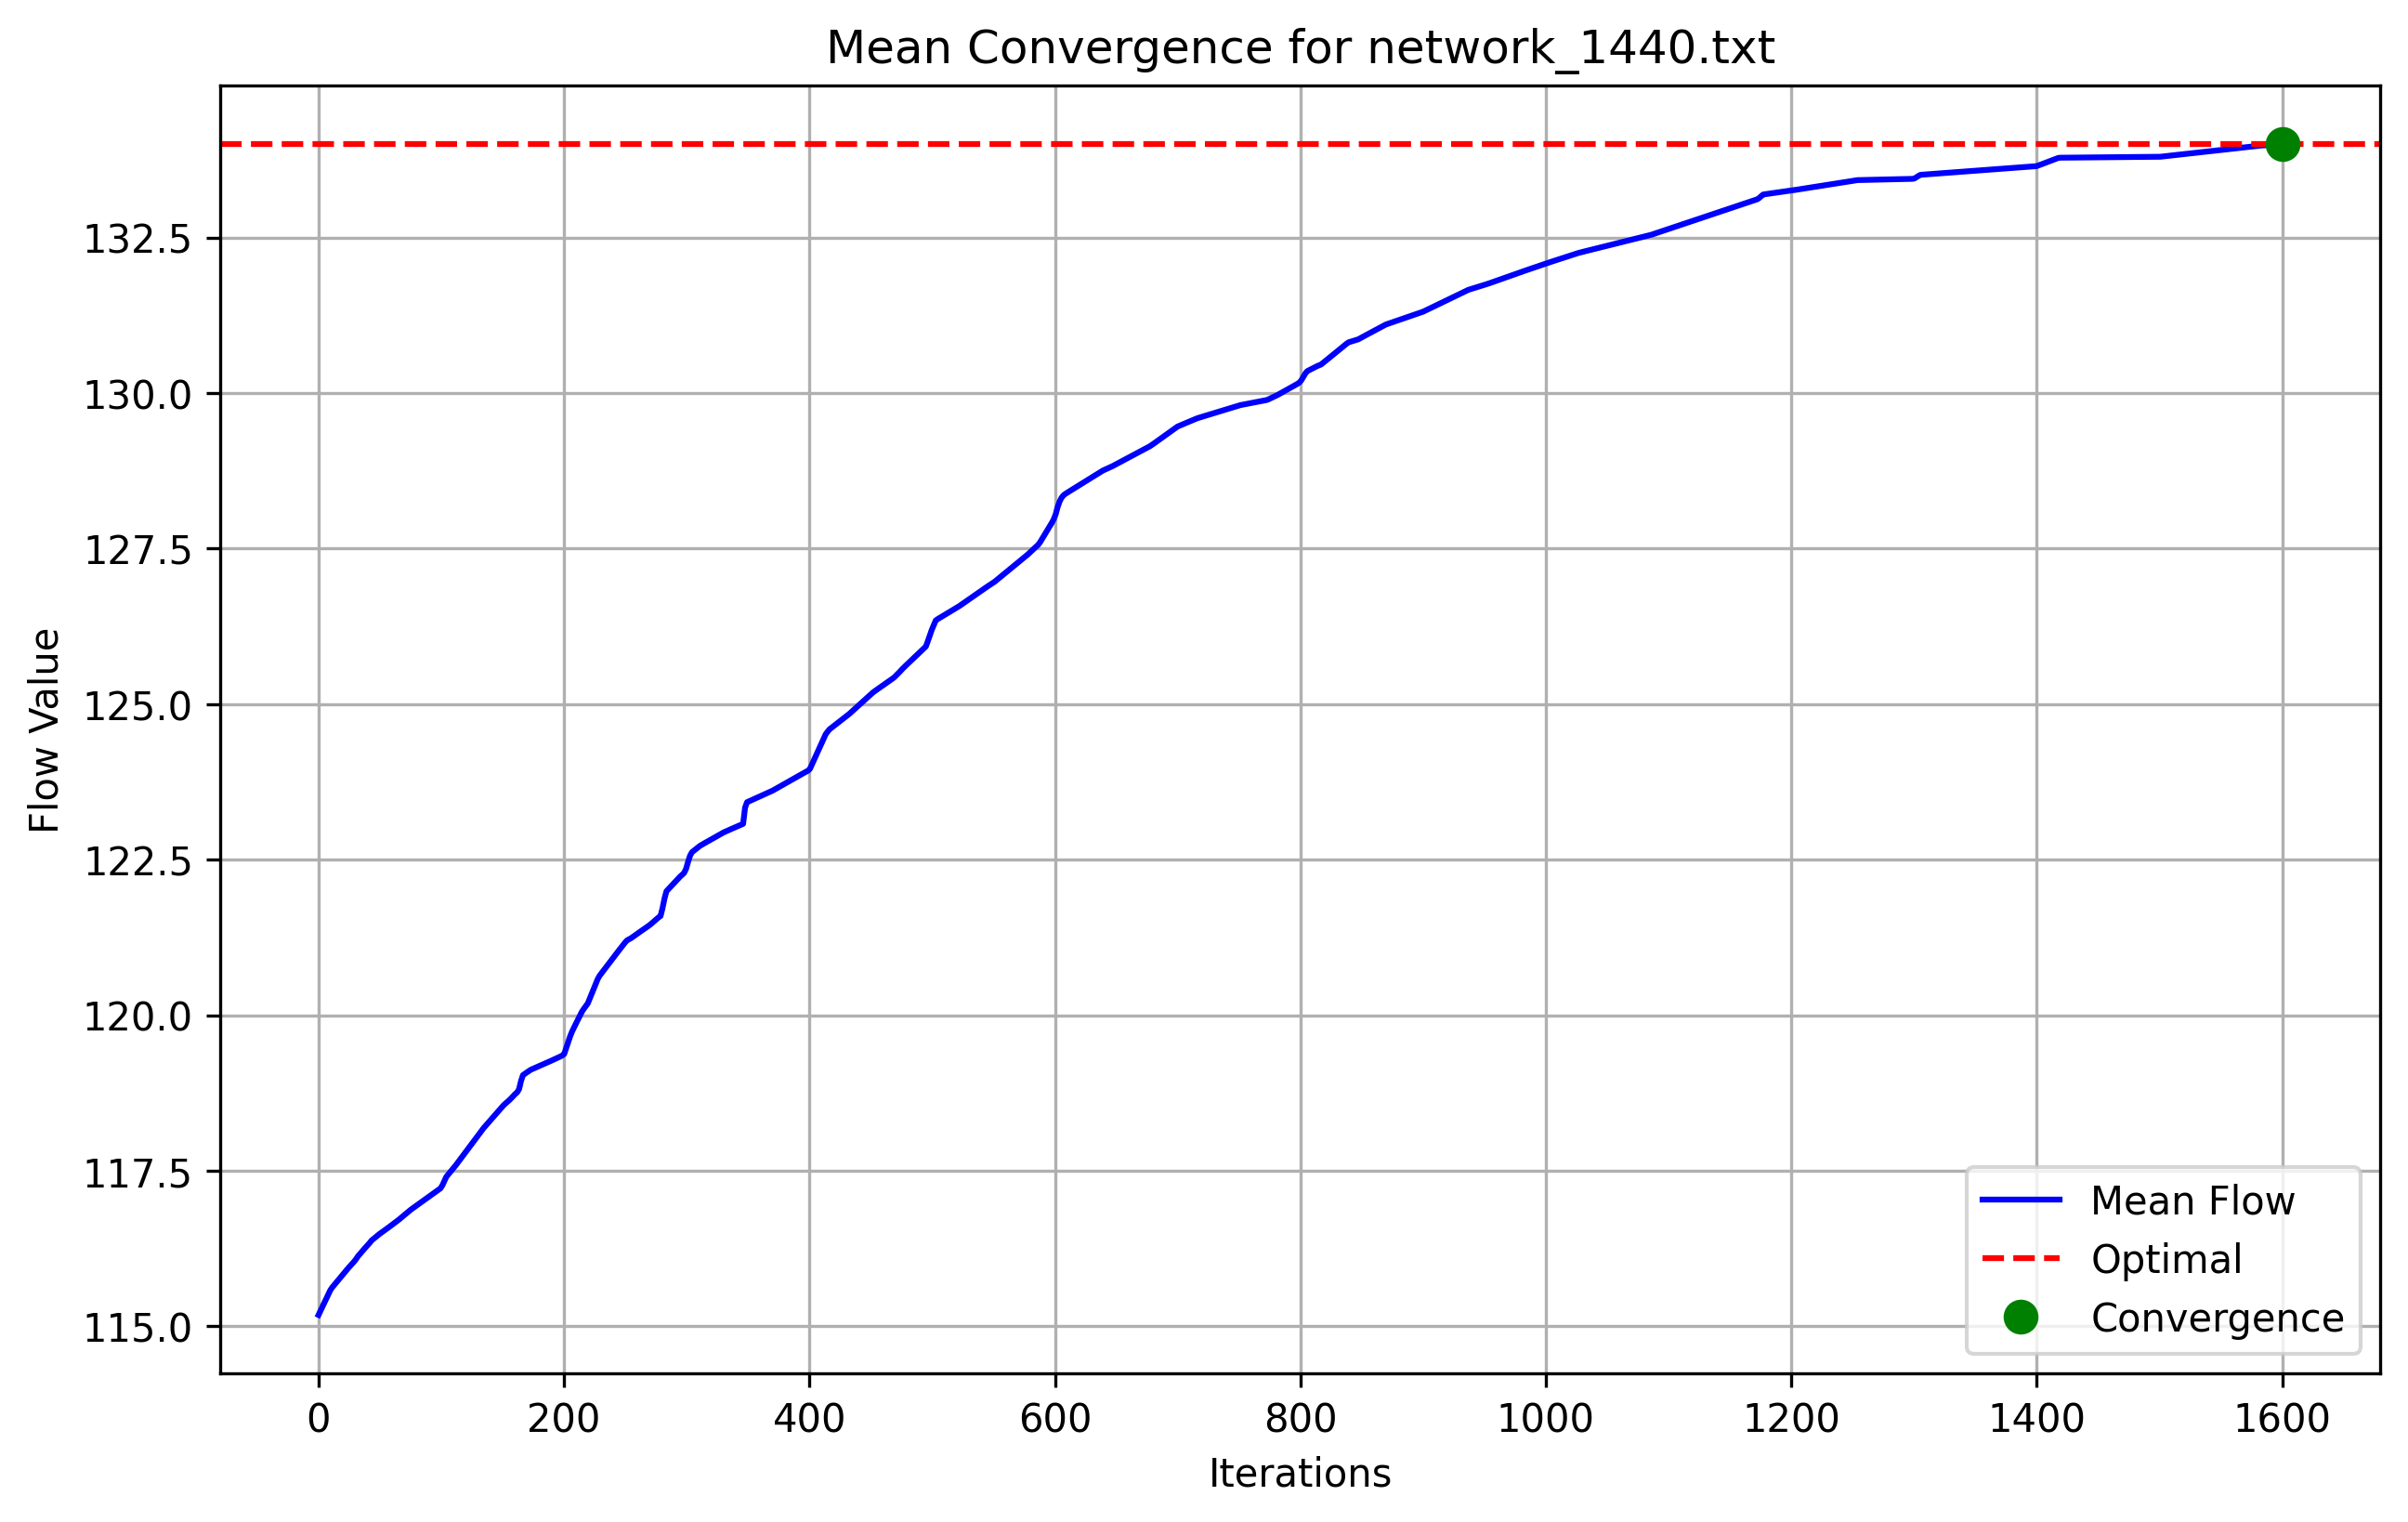
\includegraphics[width=0.8\textwidth]{results/network_1440_mean_convergence.png}
    \caption{Convergenza media per l'istanza \texttt{network\_1440.txt}.}
    \label{fig:mean_conv_1440}
\end{figure}

\begin{figure}[H]
    \centering
    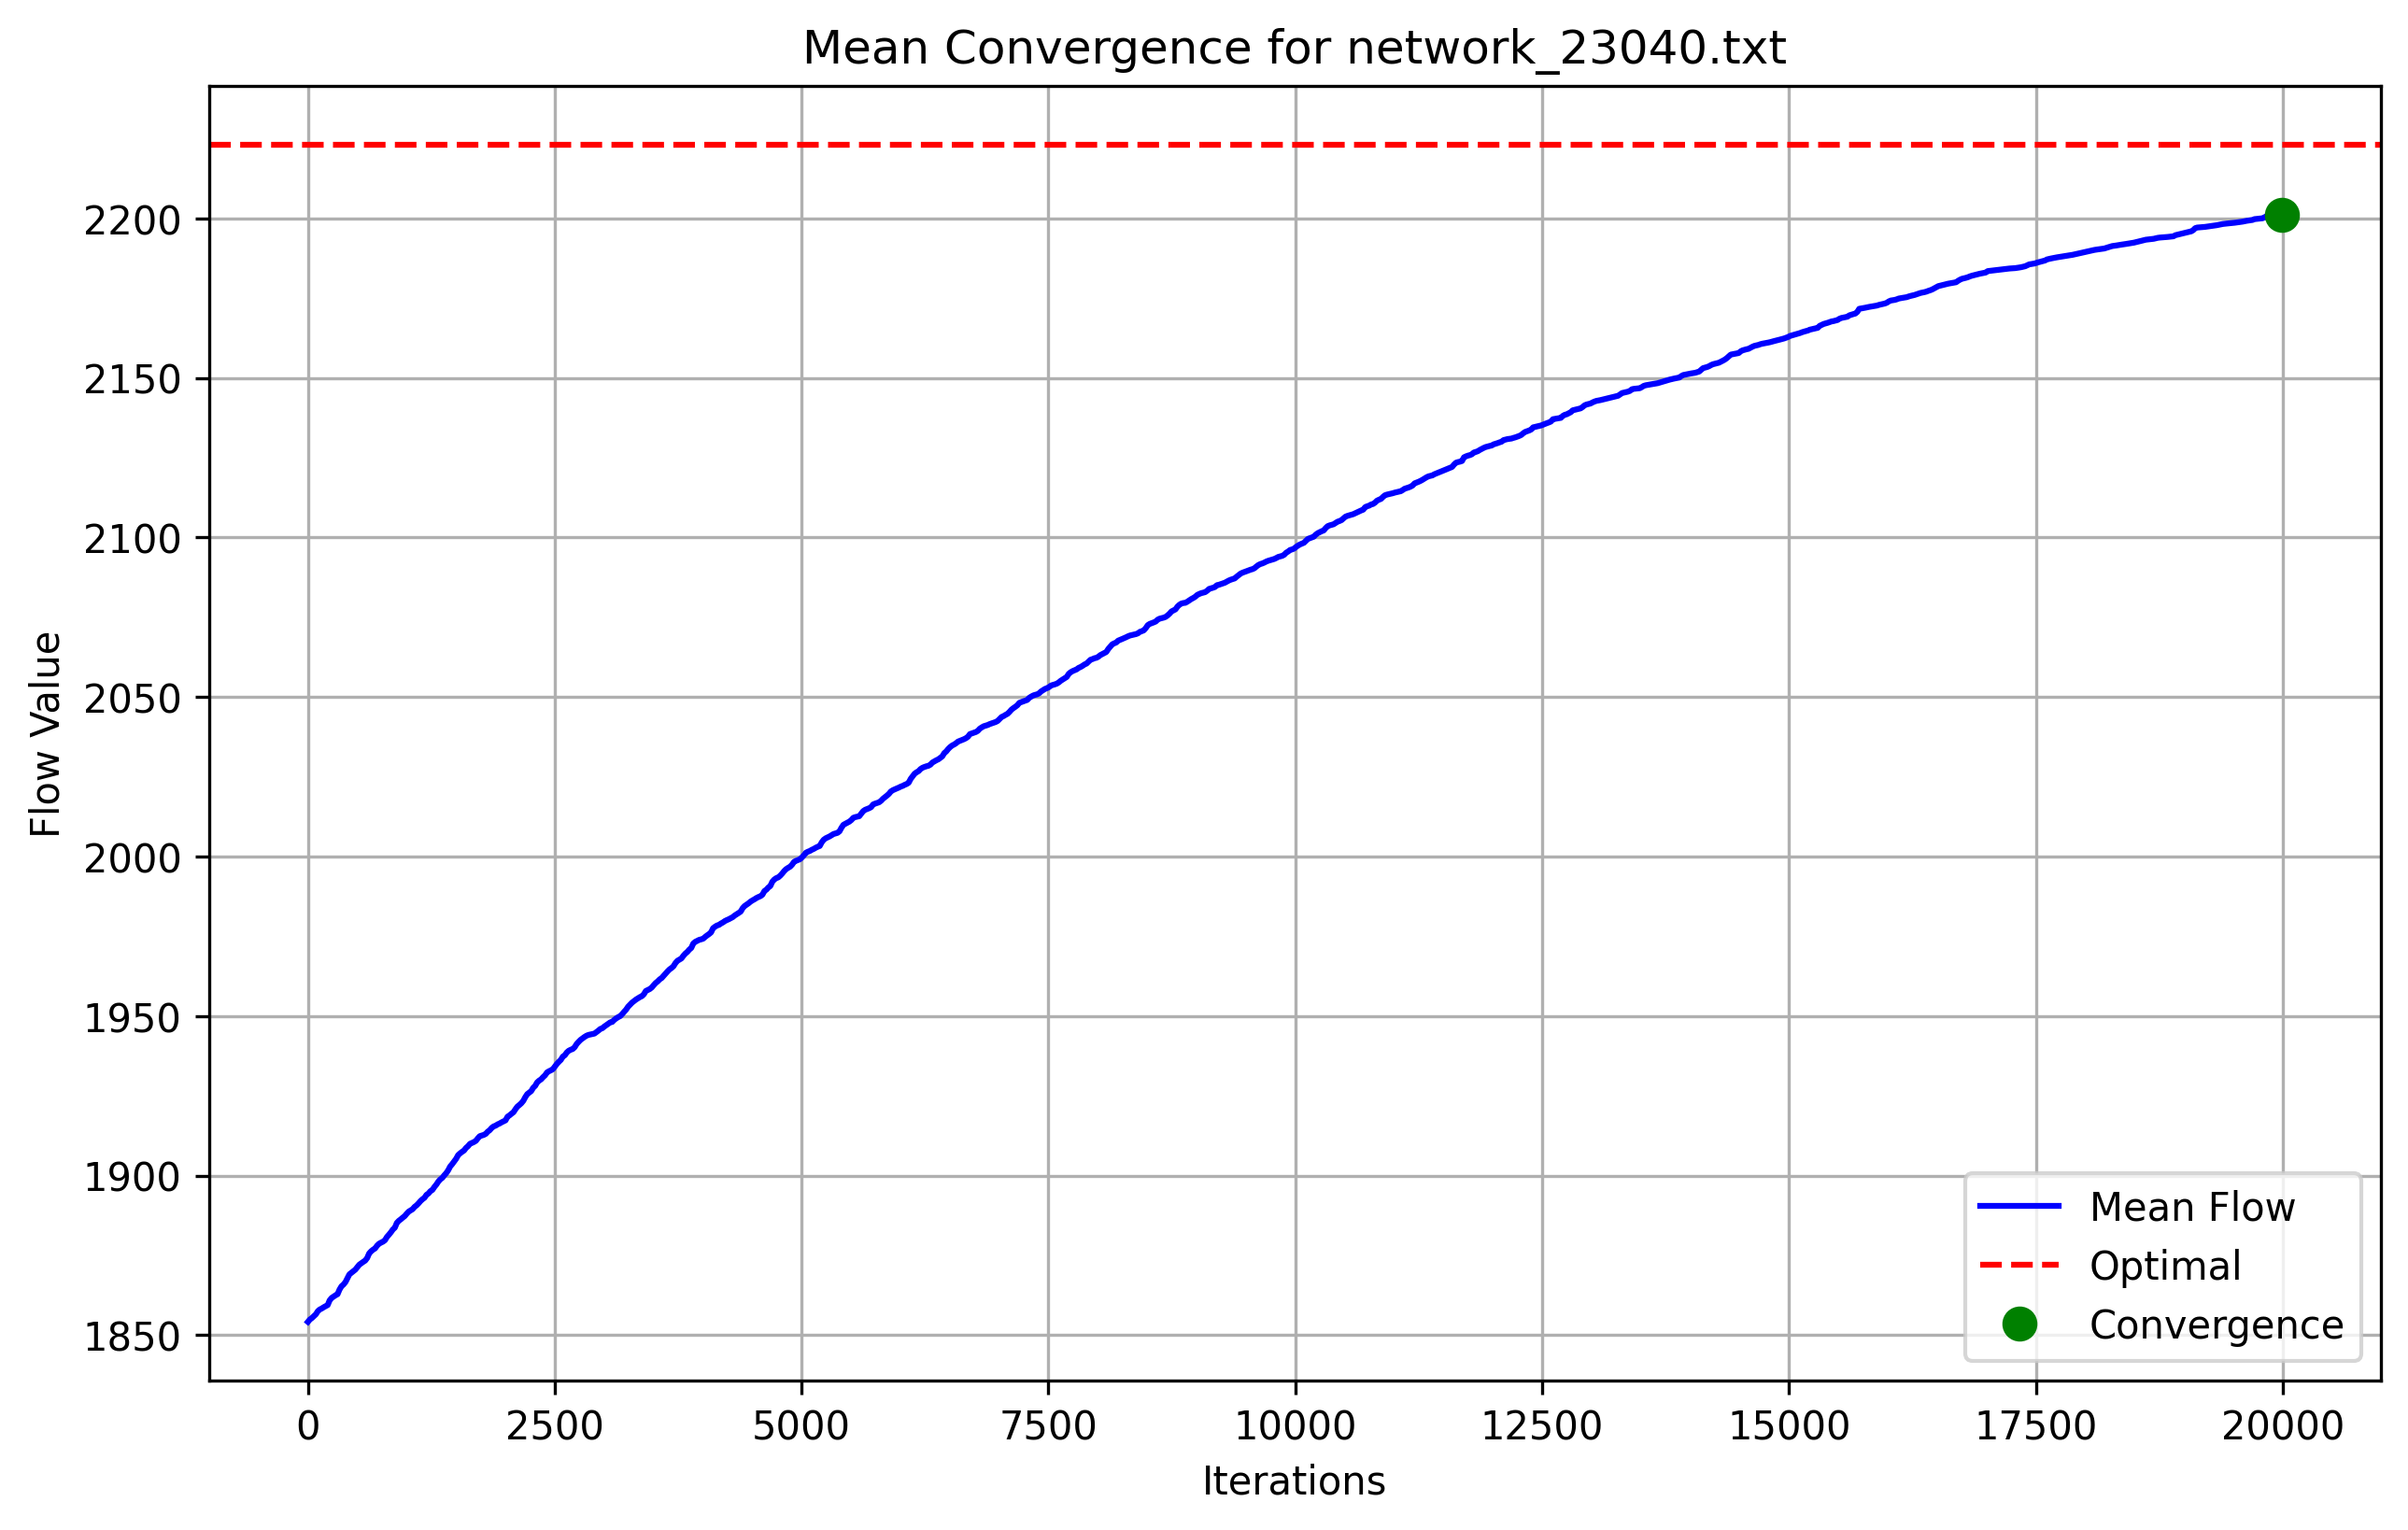
\includegraphics[width=0.8\textwidth]{results/network_23040_mean_convergence.png}
    \caption{Convergenza media per l'istanza \texttt{network\_23040.txt}.}
    \label{fig:mean_conv_23040}
\end{figure}

\section{Analisi Critica}

L’analisi critica dei risultati combina l’esame quantitativo della Tabella~\ref{tab:risultati_aggregati} con l’osservazione qualitativa dei grafici di convergenza mostrati nelle Figure~\ref{fig:best_run_1440}, \ref{fig:best_run_23040}, \ref{fig:mean_conv_1440} e \ref{fig:mean_conv_23040}. Questa doppia prospettiva permette di valutare non solo la qualità finale delle soluzioni, ma anche la dinamica del processo di ricerca.

\paragraph{Istanze di piccole e medie dimensioni}

Per istanze fino a \texttt{network\_5760.txt}, l’algoritmo mostra prestazioni eccellenti. Come evidenziato nella Tabella~\ref{tab:risultati_aggregati}, in tutti questi casi:

    
- Il \textbf{best flow} coincide esattamente con il valore ottimo.
    
- La deviazione standard è nulla, indicando che \textit{tutte le 10 esecuzioni hanno raggiunto l’ottimo}.
    
- Il numero medio di iterazioni e il tempo di esecuzione rimangono contenuti.


I grafici relativi a \texttt{network\_1440.txt} confermano questo comportamento positivo:

    
- Nella \textit{best run} (Figura~\ref{fig:best_run_1440}), l’ottimo viene raggiunto già intorno alle 800 iterazioni, con una crescita rapida e stabile del flusso.
    
- Anche la \textit{mean convergence} (Figura~\ref{fig:mean_conv_1440}) mostra una curva regolare che si avvicina all’ottimo entro 1600 iterazioni, senza lunghi plateau.


Questo dimostra che su grafi di piccole e medie dimensioni, la combinazione di vicinato ridotto, lista tabù, mosse avanzate e diversificazione controllata funziona in modo efficace ed efficiente.

\paragraph{Istanze di grandi dimensioni}

A partire da \texttt{network\_7200.txt}, emergono chiare criticità legate alla scalabilità:

    
- Per \texttt{network\_7200.txt}, la media del flusso scende a $2484.28$ (deviazione standard $\sigma = 15.97$), pur essendo l’ottimo $2502.00$.
    
- Per \texttt{network\_23040.txt}, la situazione peggiora: la media è $2201.18$ con $\sigma = 24.80$, indicando una variabilità significativa tra le esecuzioni.


I grafici di \texttt{network\_23040.txt} (Figure~\ref{fig:best_run_23040} e~\ref{fig:mean_conv_23040}) spiegano bene questo degrado:

    
- Nella \textit{best run} (Figura~\ref{fig:best_run_23040}), l’ottimo è raggiunto solo dopo circa 17500 iterazioni, evidenziando una convergenza molto lenta.
    
- La \textit{mean convergence} (Figura~\ref{fig:mean_conv_23040}) cresce in modo graduale e non raggiunge mai pienamente l’ottimo entro il budget di iterazioni.


Questi andamenti indicano che su reti molto dense:

    
- Il vicinato ridotto (circa 1–2\% degli archi) potrebbe non essere sufficiente a esplorare efficacemente lo spazio di soluzione.
    
- Le mosse locali faticano a propagare il flusso attraverso percorsi alternativi.
    
- La strategia di diversificazione, attivata ogni 2000 iterazioni, interviene troppo tardi per prevenire stagnazione prolungata.


In sintesi, mentre l’algoritmo è robusto e preciso su istanze di piccole e medie dimensioni, la sua efficienza decresce su grafi molto grandi.

\section{Conclusioni}

Il progetto ha dimostrato che il Tabu Search può essere applicato con successo al problema del massimo flusso, anche in contesti complessi e di grandi dimensioni. L’algoritmo implementato si è rivelato altamente efficace nel bilanciare qualità della soluzione, velocità di convergenza e stabilità, grazie a una combinazione ben calibrata di memoria tabù, criterio di aspirazione, diversificazione e adattività dinamica dei parametri.

I risultati sperimentali sono particolarmente incoraggianti: in 7 delle 10 istanze testate, l’algoritmo ha raggiunto sistematicamente il valore ottimo in tutte le esecuzioni. Anche nelle istanze più difficili, come \texttt{network\_23040.txt}, la soluzione media si colloca comunque entro il 99\% dell’ottimo, dimostrando una buona robustezza.

Tra le originalità introdotte, si possono evidenziare:

    
- Una \textbf{soluzione iniziale ibrida}, derivata da una versione parziale di Edmonds-Karp, che garantisce un punto di partenza di alta qualità.
    
- Un’\textbf{adattamento dinamico della tabu tenure}, che modula l’esplorazione in base al livello di stallo.
    
- Una \textbf{diversificazione controllata}, attivata periodicamente per evitare stagnazione.
    
- Un \textbf{vicinato ridotto ma mirato}, che combina efficienza computazionale e capacità di esplorazione.

In conclusione, questo lavoro mostra che le metaeuristiche possono essere competitive anche in domini tipicamente dominati da algoritmi esatti, specialmente quando si richiede flessibilità, velocità e capacità di adattamento.

\end{document}